%!TEX root = ../dissertation.tex
\chapter{The background}
\label{cap:two}
\section{Smart homes}
\newthought{Since they were released}, smartphones changed the way people do things and behave. The reason for their success was the addition of the portability feature to the computers. With portability and miniaturization of the hardware, including new sensors, which in a normal portable computer would lack usefulness, we now can fit very powerful devices into our pockets. Moreover, thanks to their sensors and interfaces, they are giving us the possibility to interact with objects in the environment, which before was not commonly defined as "smart". The interfaces we are talking about range from the wired and common \acrshort{usb}, to the wireless Bluetooth, ZigBee, Wi-Fi and so on. 
Since smartphones are changing the market and products, it is common that if we take any object in a house and search on the Internet we should find a smart version of it. There are shutter models, for instance, that are automated and can be connected to the smartphone or a smart home device, all through the Wi-Fi interface.
The widespread use of such products has developed a new discipline in computer science called the Internet of Things (IoT). 
The IoT refers to the interconnected network of physical devices, vehicles, buildings, and other items embedded with electronics, software, sensors, and connectivity, allowing these objects to connect and exchange data. IoT allows everyday objects to be connected to the Internet and to send and receive information concerning their functioning. Moreover, this connection allows for the collection and sharing of data on the device's usage and status, enabling improvements in efficiency, accuracy, and economic benefit. However, the IoT does not impact only the lives of customers. Alongside robotics, this discipline is changing the industry by directly intervening in processes or collecting useful data.
\\ Nonetheless, the focus of this thesis will be on \glspl{smarthome}, which gathers all the IoT devices that can be installed in our dwellings, and, since they are connected to the Internet, they can provide some automation to everyday actions. They include not only the shutters described above but many others, such as thermostats, TVs, and so on. 
\\ A study \cite{s21113838} shows how the pandemic changes the way we live, in particular inside our homes. In fact, people and companies are adopting the work from home, as such people who are not in the office all day, are experiencing changes in their home, in order to make them not only a better place to live, but also to be productive. The reasons why someone wants to buy a smart device can range from economic reasons, such as saving money and energy, to security or health reasons. A study on the benefits and risks of smart home devices \cite{wilson2017benefits}, conducted on a sample of a hundred people in the UK, shows what customers think are the main benefits of having one of them installed at home (fig. \ref{graph:smart-reas}). 
\begin{figure}[ht]
    \centering
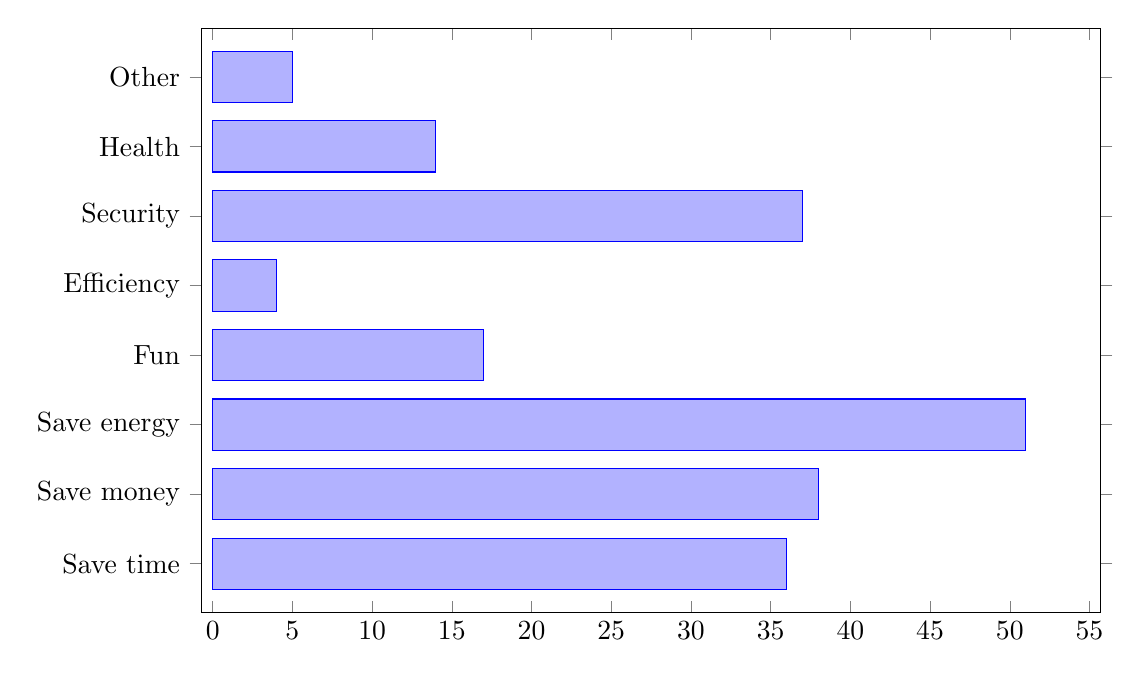
\begin{tikzpicture}
  \begin{axis}[
    enlargelimits=true,
    height=9cm,width=13cm,
    bar width=0.65cm,
    symbolic y coords={{Save time}, {Save money}, {Save energy}, Fun, Efficiency, Security, Health, Other},
    xbar
    ]
    \addplot coordinates { (36,{Save time}) (38,{Save money}) 
		(51,{Save energy}) (17,Fun) (4,Efficiency) (37,Security) (14,Health) (5,Other) };
  \end{axis}
\end{tikzpicture}
\caption{Histogram showing the frequency of responses to the question "How do prospective users perceive the specific benefits and risks of smart home technologies?" on a sample of a hundred people in the UK \cite{wilson2017benefits}.  }
\label{graph:smart-reas}
\end{figure}
Therefore, it is not surprising that we are talking about a large and constantly growing market in which many companies are investing. 
\section{Smart-locks}
Locks and keys, as we know them today, have not changed much since they were invented. A lock is installed inside the door profile and a deadbolt can fit a key with a specific shape, which turning can enable or disable the lock. This solution, with a few variations, has remained unchanged through the era, since it actually fits the purpose. However, the advent of \acrshort{IoT} raises the question of whether having physical keys is always a benefit in terms of security. Keys until now were the best solution to prevent unwanted people from accessing a private property, but they can be stolen and cloned, even from the deadbolt shape. 
\\ As such, door lock manufacturers start to produce new models with a wireless interface, which drives their interest in the IoT market. The proposed solutions are really different from each other, due to the number of possible implementation and hardware involved, such as keypad, deadbolt, handle, fingerprint and so on; and even due to the type of interfaces, such as Bluetooth, ZigBee, \acrshort{nfc}, Wi-Fi.
A customer who experiences the purchase of this type of product must face a variety of devices, each with different technologies, and has to choose the one that fits his needs. Even the installation method, for example whether the device can operate with the existing lock or not, could be a discriminating factor. As such, this market is fragmented and there are many products that are spreading through it. 

\subsection{Smart-lock interfaces}
A smart-lock, as it is intended in this thesis, \emph{is an electromechanical device that performs locking/unlocking operations of a door, after receiving the command through a wireless interface.} \\
The emphasis on the wireless nature of a smart-lock is mandatory for us, since some definitions do not include this particular characteristic, as a consequence involving devices that are not in our interest. 
\\ The following types of smart locks differ from each other by the type of wireless interface used.
In particular, what is required in this context are the following features.
\begin{itemize}
    \item High reliability, which can be translated into low power consumption. Smart-locks are usually based on lithium batteries, as such they are not connected to a stable power line. A wireless technology has always to deal with a standby power consumption value, which in this case must be low.
    \item Low cost: these devices are not usually cheap, but they have to reach a consumer market, in order to spread as much as possible. 
    \item Secure: the implementation of a safe communication channel is a priority when we are considering a device which is designed to protect the home accesses. The focus is on the wireless protocol used to communicate, which must be secured and implemented with encryption.
\end{itemize}
The following wireless interfaces list are not complete, there are many other interfaces, like NFC, fingerprint and so on. They can be neglected, because they are not more widespread than the one presented or relevant for the purpose of the project. Moreover, it must be specified that smart-locks use not only an interface, but they usually use hybrid wireless connections of the following.
\subsubsection{Bluetooth}
Bluetooth is the commercial name of the standard \acrshort{ieee} 802.15.1, for short-range wireless technology. The protocol architecture can be divided into different layers. 
\begin{itemize}
    \item The core protocols are the low level management system, including, for example, the radio interface, the link manager protocol, which assures authentication, encryption and other security features.
    \item The cable replacement and telephony control are emulation protocols over the \gls{l2cap} which provides an interface for each of the high level protocols. 
    \item Other existing protocols, such as \acrshort{tcpip}, which are customized to communicate with L2CAP. 
\end{itemize}
\begin{figure}[ht]
    \centering
    \includegraphics[width=\textwidth]{figures/bluetooth-arch.png}
    \caption{Bluetooth Protocol Stack.}
    \label{fig:blueetooth}
\end{figure}
Despite its age, Bluetooth is gaining popularity, especially in the last decade, with the spread of wireless devices, such as headphones, because it provides low latency. The main purpose of this technology is the wire replacement, but in the various updates, many other features have been added, like, for example, the possibility of internet bridging. Another important characteristic is that Bluetooth is designed to be low cost, eventually under \$10/unit \cite{1007414}. It assures a communication range of 10 meters, which is more than sufficient if we do not need remote control on the device. Finally, the telephony control protocol allows connected devices to handle both data and voice transmission. This is the main reason why a Bluetooth module is now installed in most smartphones.
\\ As such, many smart locks usually implement Bluetooth, because it meets all its requirements. The biggest limitation of this particular approach is the lack of remote control capability. The short-range nature of the protocol does not allow communication over 10 meters, and, to patch up this limitation, information must be forwarded by a bridge connected to \acrlong{www}.

\subsubsection{Zigbee}
\gls{ieee} 802.15.4 is a standard released in 2004 for a low-rate wireless network. The characteristics of this technology could be summarized as follows \cite{5942102}.
\begin{itemize}
    \item Reliable and self-healing.
    \item Supports a large number of nodes.
    \item Secure, with standards based security [AES128].
    \item Low cost.
    \item Low power (ability to operate on batteries
    measured in years).
    \item Low maintenance (meshing, self organizing).
\end{itemize}
Part of these goals are reached through the Direct Sequence Spread Spectrum (DSSS) modulation technique, which grants a range up to 150 meters and a low power consumption, compared to the Frequency Hopping Spread Spectrum (FHSS), used by other technologies, including Bluetooth.
Zigbee devices are usually organized on a network with a coordinator at the center, who is responsible for the initialization of the channels and security parameters. Moreover, it is the component in charge of bridging to other networks type. 
\\ Then, there is the router, which acts as an intermediate node, accepting connections from the other devices and retransmitting to the receiver. Finally, the end devices are the ones operating actions, with sensors and switches. 
\\ Thanks to the technologies in use and the specific radio frequencies chosen, Zigbee devices can rely on batteries and last for years, due to the incredible low power consumption achieved in standby. We must not forget that IoT devices are in standby most of the time and the latent consumption must be lower than possible. 
\\ The performance of this technology is overall better than that of Bluetooth; however, Zigbee presents a non-negligible limitation, which is the absence of the dedicated modem inside almost all smartphones. Although Bluetooth is widespread in the consumer market, thanks to its integration inside smartphones, ZigBee can rely only on the smart home implementation, when it is supported. A ZigBee smart home configuration usually has various sensors as nodes and a central server which acts as controller and it bridges to another network, which are commonly Wi-Fi or Ethernet. Only then, from the latter network, the user applications can interface with the ZigBee devices.
\\ In the case of smart-locks, the ZigBee interface, if implemented, is not used to operate directly with a smartphone, but to share information about access with the smart home application. However, communication can even occur, but must be bridged through another network to which the smartphone can connect, such as Bluetooth or Wi-Fi. 
\subsubsection{Wi-Fi}
Wi-Fi is the name of a family of standards with the official name of IEEE 802.11. Wi-Fi technologies are commonly used to provide a wireless access point for the Internet, since they usually operate in WLAN. It is the most widespread wireless technology in the consumer market and the reasons for that are various. First of all, it supports high bandwidth, up to 600 Mbps with 2.4 Ghz frequency spectrum and 1.3 Gbps with 5 Ghz. Moreover, it is reliable, secure and its signal can reach high distances, for instance some of its extensions can reach 1 km of range. 
\\ Most mobile devices that connect to the Internet have a Wi-Fi modem inside, including smartphones. As such, it is always the primary choice when building a smart home that allows devices to communicate through its dedicated modem. This scenario is justified by the fact that Wi-Fi exists, in most houses, before the spread of the IoT, for internet connection purposes. As such, most IoT devices and the relative application communicate over a Wi-Fi network, which provides an eventual internet connection. 
\\ Smart-locks connected to the Wi-Fi are usually remotely controllable. In fact, Internet access makes these devices available by \acrshort{http} requests over \acrshort{www}.
\\ From a security point of view, Wi-Fi provides different options. Most access points provide an authentication system with the \acrshort{wpa2psk} protocol, which also allows the network to identify the connected devices. Furthermore, having access to the HTTP protocol allows applications to implement its security protocols, such as \gls{tls}. 
However, the use of Wi-Fi technologies can have downsides. For example, power consumption is much higher than in previous technologies. This is usually a problem with mobile devices that are powered by batteries and not connected to a power line. In the IoT, this could be bypassed in some ways, like using hybrid approaches. Many smart-locks, for example, use external bridges that can be connected to the power socket and communicate to the hardware with Bluetooth. As such, the smart-locks uses a low power protocol to communicate with the bridge and the latter forward the data to the home server. Moreover, with the development of these protocols, power consumption has taken many steps forward. Bluetooth, for example, to fill the concurrency gap, has developed a low-power version, called \gls{ble}. BLE is able to consume less power approaching the communication with a client-server architecture, using smaller packet, improving the idle time with a sleeping mode and better managing the frequencies in use. Even Wi-Fi has recently introduced new protocols, such as the Target Wake Time (TWT), which improves the wake-up time scheduling of the devices.
\\ It is important to specify that the values in the below table \ref{tab:wireless-compare} are referring to older, but widespread implementations of the protocols. However, this table is useful for giving an idea of the overall differences between the technologies. 

\begin{table}[ht]
\def\arraystretch{1.75}
\begin{tabular}{|l|lll|}
\hline
Standard            & Bluetooth & ZigBee      & WiFi    \\
\hline
\hline
Chipset             & BlueCore2 & ZigBee Chip & CX5311  \\
\hline
Range (m)           & 10        & 40-100      & 100     \\
\hline
VDD (volt)          & 1.8       & 2.4-3.4     & 3.3     \\
\hline
Bit rate (Mbps)     & 0.72      & 0.25        & 52      \\
\hline
Battery Life (days) & 1 - 7     & 100 - 1000  & 0.5 - 5 \\ [1ex] 
 \hline
\end{tabular}
\caption{Comparison of wireless technologies, focusing on power consumption and performance in the context of smart grid communication. \cite{7030564}}
\label{tab:wireless-compare}
\end{table}

\subsection{Smart-locks network design}
\label{sec:dgcsmartlocks}
Comparing the various solution proposed by the manufacturer, it is possible to identify a common pattern on how smartphone and smart-lock communicate. The most popular is the Device-Gateway-Cloud model \cite{10.1145/2897845.2897886} (fig. \ref{fig:dgc}), in which the smartphone pairing acts as a gateway to the Internet sending the information to the provider server. This is forced by the lack of a Wi-Fi modem in most smart-lock solutions. However, if it is able to connect to the home network, smart-lock and server can communicate directly, as such the state updates are transmitted through the internet connection. 

\begin{figure}[ht]
    \centering
    \includegraphics[width=\textwidth]{figures/dgc.png}
    \caption{The Device-Gateway-Cloud model, the smart-lock use the smartphone as a gateway to the server.}
    \label{fig:dgc}
\end{figure}

\subsection{Smart-lock application}
\label{sec:smart-app}
The mobile application, installed in the smartphone, plays an essential role in smart-lock management. As we mentioned in the Device-Gateway-Cloud model, the application is responsible to collect data from the device and sent in to the cloud. Moreover, it is able to send request, like the unlock/lock one, to the smart-lock and listen to the answer. Most of the applications provided by the smart-lock manufacturer run on Bluetooth, and as such, the first communication between device and smartphone must be preceded by the pairing of the two. Pairing sets the wireless connection and, most of the time, creates a handshake key that grants communication even offline. 
\\ The unlocking process could be slightly different, depending on the smart-lock model. Some of the devices have to be physically touched and if the smartphone paired is in the Bluetooth range, it will unlock. Some others have a virtual button inside the application and do not expose any hardware to the exterior. 
\\ Moreover, within the app, the access log list is usually available, which is particularly useful in this context. Through this feature, the application can show the usage history of a key and see who is entered in the house, as such it can also detect the unexpected access.
\\ Finally, the killer feature is the possibility to generate virtual keys that can abstract different access levels in complex systems, or simply can generate temporary permissions.

\subsection{Smart-lock vulnerabilities}
\label{sec:smartlockvulnerabilities}
Because of the importance of the subject, the literature is treating smart-lock device security issues with particular attention. A possible spreading of this technology in everyone's homes could be a new opportunity for new cyber-thieves, which want to break into not them properties. 
Sometimes, vulnerabilities are based on device design, so it is very important to discover these defects during their analysis. 
For example, a basic type of attack could affect the hardware directly. We all know that tech gadgets most of the time are not built to resist, for various reasons, from the maintenance one to the production costs. As such, it is better that a smart-lock does not expose any mechanical part to the outside face of the door. Otherwise, anyone could have access to the device, understand the model and act accordingly. 
\\ However, due to the design of a smart-lock, it is never possible to hide the hardware. As such, we can only analyze software vulnerabilities.

\subsubsection{Architectural attacks}
This type of attacks can be executed remotely because they rely on architectural vulnerability, in particular in communication between the gateway and the server. 

\paragraph{Man-In-The-Middle attacks}
This type of attack can be performed by routing the communication flow through a malicious proxy by changing the API URL parameter, which is the server address to which the smartphone application is connecting\cite{mitm}. As such, the entire data passing through the proxy can be read and the proxy can even fake the response to the application. This can still happen in a system using certificates signing the software involved, because the application does not know that the server to which it is connecting is a proxy. As such, it keeps sending the certificate, which can be easily forwarded to the real server by proxy, leaving no trace. 

\paragraph{Overpriviledge attacks}
Many smart-lock manufacturers expose public \acrshort{api} to third-party developers. This is not only a benefit for who is integrating the smart-lock functionality, but even for the provider, can have positive effects, such as a better user experience, thanks to a richer ecosystem.
\\ However, this approach can expose a critical part of the system to software that is not under the control of the manufacturer. In fact, most of the APIs are accessible with OAuth authentication flows, which require a client ID to prove the identity. In the case that a developer lets this client ID be in plain text, accessible with a simple code inspection, this can represent a serious vulnerability.
\\ This category includes attacks that can be performed on bad design APIs by the manufacturer itself. That can happen if a third-party application is requesting a type of privileges, for example, reading the status of the battery, but the bad designed library gives them access to resources which are not requested, or worse, are meant to be hidden.\cite{7546527}

\paragraph{Eventual consistency}
Eventual consistency verifies when data in the smart-lock application and the server must remain continuously synchronized. This is a problem, especially in the Device-Gateway-Cloud model, where the smart-lock state in the server is a projection of the state on the application. In this type of architecture, the two states must be synchronized or the system can accused vulnerabilities. For example, if the owner creates a one time key, giving permission to a temporary guest, and then he/she revokes the permission on the key, if the guest smartphone is not reachable, because he/she can simply had disabled the internet connection, the server can not revoke the permission. As such, the guest application can still have access until the connection is restored and the synchronization is available again. \cite{10.1145/2897845.2897886}

\subsubsection{Application attacks}
Most of the time, the mobile application is the vital part of the system. As such, its vulnerabilities are serious points of failure. In particular, are not uncommon attacks on the communication between the application and the smartphone. 
\\ As mentioned in section \ref{sec:smart-app}, most applications use a Handshake Key, in order to establish a connection between the smartphone and the smart-lock. In the mobile operating system, there are many ways to access sensitive information from the application. One can be using a rooted/jailbroken operating system in which the smartphone owner acts as a superuser, so that he/she is able to access the storage of the device and see protected data. As has been shown in other works\cite{8116427}, the Handshake Key can be stolen simply by accessing a \acrshort{xml} file from the manufacturer application.  

\paragraph{Denial of Service (DoS)}
With the possibility of controlling communication between the smartphone and the smart-lock, the attacker can disable the functionality of the device. It has been shown that if a smart-lock can handle only a Bluetooth connection at the time and there is no priority system, the attacker can continuously send link request to the device, preventing the owner/user to connect with its application\cite{8116427}. 

\paragraph{Storage attacks}
We have described above how to steal the Handshake Key. However, with the same method, it is possible in some cases to steal even personal information from the application storage. That happens primarily because of the application developers fault, which are letting the data save without encryption.

\subsubsection{Preventing the attacks}
As we can see in the above sections, most of the fault, of the vulnerability presence, relies on developers' care. Sometimes a well-designed system is enough, in order to prevent unnecessary information to arrive in the wrong hands. However, when this is not possible, especially in application mobile storage, it is always the best practice using a state-of-the-art crypto-system, in order to protect the sensible data.
\\ Smart-locks, thanks to theirs features, can even been improved with more security layers by design. Some of the manufacturer applications are able to use the GPS location of the user and determine if he/she is in the near the device (geo-fencing). With this system is easy to prevent malicious application to win too easy the unlocking challenge.  